%%%%%%%%%%%%%%%%%%%%%%%%%%%%%%%%%%%%
% Slide options
%%%%%%%%%%%%%%%%%%%%%%%%%%%%%%%%%%%%

% Option 1: Slides with solutions

\documentclass[slidestop,compress,mathserif]{beamer}
\newcommand{\soln}[1]{\textit{#1}}
\newcommand{\solnGr}[1]{#1}

% Option 2: Handouts without solutions

%\documentclass[11pt,containsverbatim,handout]{beamer}
%\usepackage{pgfpages}
%\pgfpagesuselayout{4 on 1}[letterpaper,landscape,border shrink=5mm]
%\newcommand{\soln}[1]{ }
%\newcommand{\solnGr}{ }


%%%%%%%%%%%%%%%%%%%%%%%%%%%%%%%%%%%%
% Style
%%%%%%%%%%%%%%%%%%%%%%%%%%%%%%%%%%%%

\def\chp4@path{../../Chp 4}
\input{../../lec_style.tex}


%%%%%%%%%%%%%%%%%%%%%%%%%%%%%%%%%%%%
% Preamble
%%%%%%%%%%%%%%%%%%%%%%%%%%%%%%%%%%%%

\title[Lecture 11]{MA213: Lecture 11}
\subtitle{Module 2: Probability, Random Variables, and Distributions}
\author{OpenIntro Statistics, 4th Edition}
\institute{$\:$ \\ {\footnotesize Based on slides developed by Mine \c{C}etinkaya-Rundel of OpenIntro. \\
The slides may be copied, edited, and/or shared via the \webLink{http://creativecommons.org/licenses/by-sa/3.0/us/}{CC BY-SA license.} \\
Some images may be included under fair use guidelines (educational purposes).}}
\date{}

%%%%%%%%%%%%%%%%%%%%%%%%%%%%%%%%%%%%
% Begin document
%%%%%%%%%%%%%%%%%%%%%%%%%%%%%%%%%%%%

\begin{document}


%%%%%%%%%%%%%%%%%%%%%%%%%%%%%%%%%%%%
% Title page
%%%%%%%%%%%%%%%%%%%%%%%%%%%%%%%%%%%%

{
\addtocounter{framenumber}{-1} 
{\removepagenumbers 
\usebackgroundtemplate{\includegraphics[width=\paperwidth]{../../OpenIntro_Grid_4_3-01.jpg}}
\begin{frame}

\hfill \includegraphics[width=20mm]{../../oiLogo_highres}

\titlepage

\end{frame}
}
}


%%%%%%%%%%%%%%%%%%%%%%%%%%%%%%%%%%%%
% Recap/Agenda 
%%%%%%%%%%%%%%%%%%%%%%%%%%%%%%%%%%%%
% TODO better formatting
\begin{frame}
    \frametitle{Module 2: Probability, Random Variables, and Distributions}
    \begin{itemize}
        \item \hl{Previously: } Normal distribution (Chapter 4.1)
        \item \hl{This time: } Normal distribution, continued
        \item \hl{Reading: } Chapter 4.2 for next time
        \item \hl{Deadlines/Announcements: } HW 4 due Monday
    \end{itemize}
    
\end{frame}
    
%%%%%%%%%%%%%%%%%%%%%%%%%%%%%%%%%%%%
% Learning objectives:
%%%%%%%%%%%%%%%%%%%%%%%%%%%%%%%%%%%%
\begin{frame}
    \frametitle{Learning Objectives}
    \begin{itemize}
        \item \textbf{M1 LO3: Use R for Data Management and Exploration:} Utilize R to load, pre-process, and explore data through visualization and summarization techniques.
        \item \textbf{M2 LO1: Validate and Explain Probability Distributions:} Assess the validity of a probability distribution using the concepts of outcome, sample space, and probability properties (e.g., disjoint outcomes, probabilities between 0 and 1, and total probabilities summing to 1).
        \item \textbf{M2 LO3: Compute Probabilities Using Various Tools:} Use logic, Venn diagrams, and probability rules to compute probabilities for events.
        \item \textbf{M2 LO4: Understand and Compute Expectations and Variances:} Explain the concepts of expectations and variances of random variables, and compute the expectation and variance of a linear combination of random variables.
        \item \textbf{M2 LO6: Assess Data Using the Normal Distribution:} Use the normal distribution to assess the "unusualness" of data points, apply the 68-95-99.7% rule, evaluate normality through histograms and q-q plots, and determine when a normal approximation to the binomial model is valid for calculating binomial probabilities.
    \end{itemize}
\end{frame}


%%%%%%%%%%%%%%%%%%%%%%%%%%%%%%%%%%%%
% Sections
%%%%%%%%%%%%%%%%%%%%%%%%%%%%%%%%%%%%

\section{Normal distribution, continued}

%%%%%%%%%%%%%%%%%%%%%%%%%%%%%%%%%%%

\subsection{68-95-99.7 rule}

%%%%%%%%%%%%%%%%%%%%%%%%%%%%%%%%%%%%

\begin{frame}
\frametitle{68-95-99.7 Rule}

\begin{itemize}

\item For nearly normally distributed data, 
\begin{itemize}
\item about 68\% falls within 1 SD of the mean,
\item about 95\% falls within 2 SD of the mean,
\item about 99.7\% falls within 3 SD of the mean.
\end{itemize}

\item It is possible for observations to fall 4, 5, or more standard deviations away from the mean, but these occurrences are very rare if the data are nearly normal.

\end{itemize}

\begin{center}
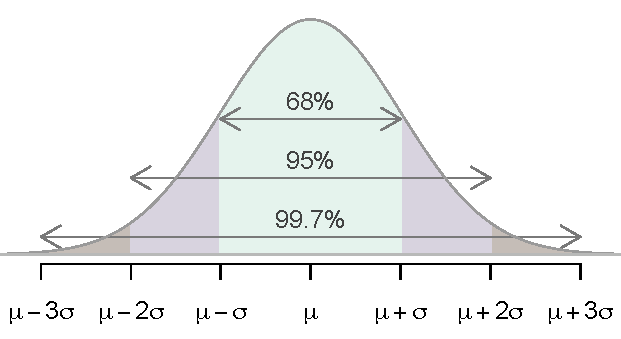
\includegraphics[width=0.7\textwidth]{\chp4@path/4-1_normal_distribution/figures/6895997/6895997}
\end{center}

\end{frame}

%%%%%%%%%%%%%%%%%%%%%%%%%%%%%%%%%%%%

\begin{frame}
\frametitle{Describing variability using the 68-95-99.7 Rule}

SAT scores are distributed nearly normally with mean 1500 and standard deviation 300.

\pause
\begin{itemize}

\item $\sim$68\% of students score between 1200 and 1800 on the SAT. 

\item $\sim$95\% of students score between 900 and 2100 on the SAT. 

\item $\sim$99.7\% of students score between 600 and 2400 on the SAT. 

\end{itemize}

\begin{center}
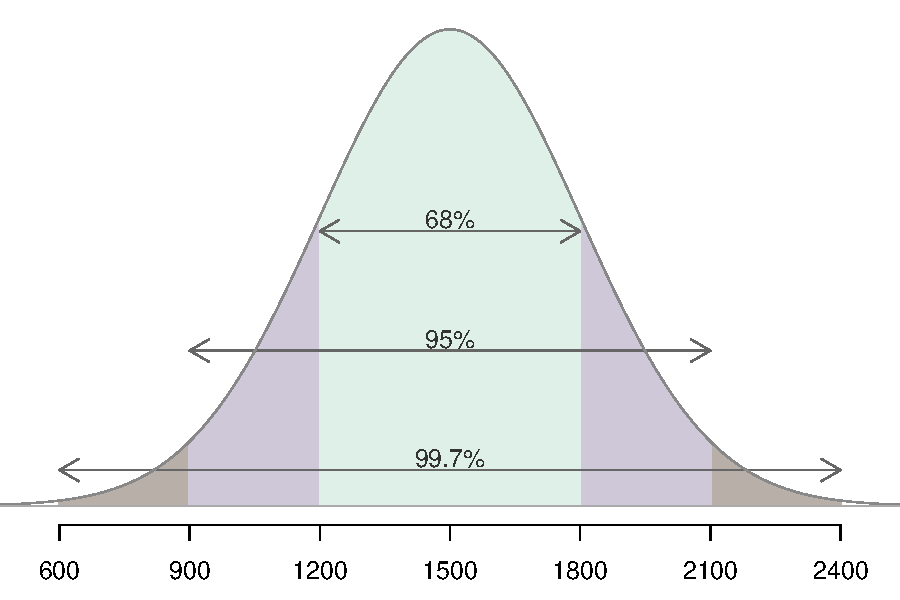
\includegraphics[width=0.65\textwidth]{\chp4@path/4-1_normal_distribution/figures/sat_empirical/sat_empirical}
\end{center}

\end{frame}

%%%%%%%%%%%%%%%%%%%%%%%%%%%%%%%%%%%%

\begin{frame}[fragile]
\frametitle{Number of hours of sleep on school nights}

\only<1 | handout:0>{
\begin{center}
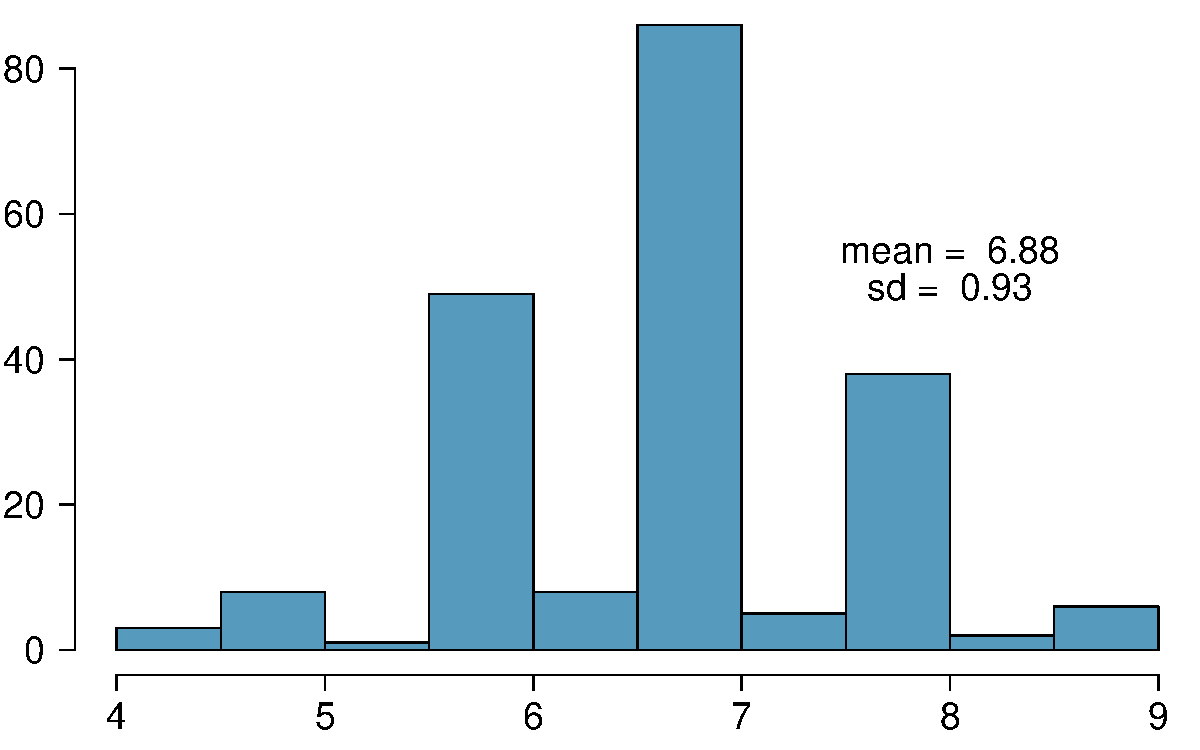
\includegraphics[width=0.75\textwidth]{\chp4@path/4-1_normal_distribution/figures/sleep/sleep-hist} 
\end{center}
\vspace{-0.25cm}
\begin{itemize}
\item Mean = 6.88 hours, SD = 0.92 hrs
\item[] \textcolor{white}{72\% of the data are within 1 SD of the mean: $6.88 \pm 0.93$}
\item[] \textcolor{white}{92\% of the data are within 2 SD of the mean: $6.88 \pm 2 \times 0.93$}
\item[] \textcolor{white}{99\% of the data are within 3 SD of the mean: $6.88 \pm 3 \times 0.93$}
\end{itemize}
}

\only<2 | handout:0>{
\begin{center}
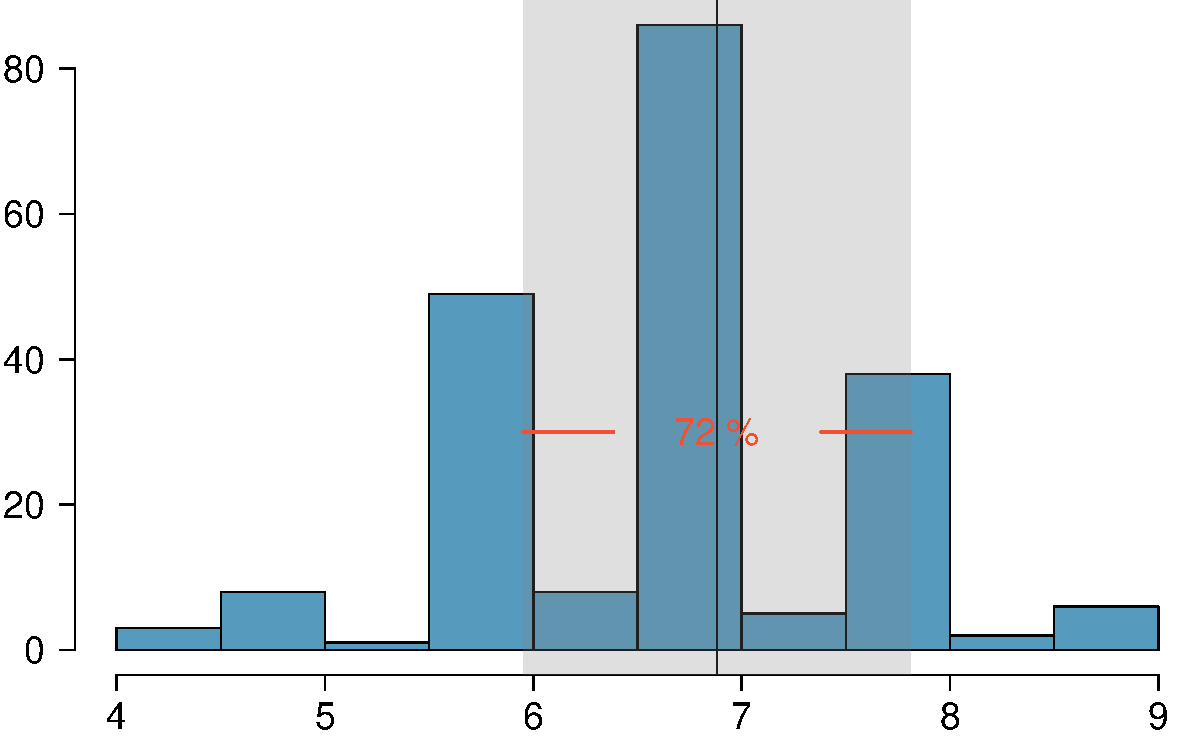
\includegraphics[width=0.75\textwidth]{\chp4@path/4-1_normal_distribution/figures/sleep/sleep-hist-sd1} 
\end{center}
\vspace{-0.25cm}
\begin{itemize}
\item Mean = 6.88 hours, SD = 0.92 hrs
\item 72\% of the data are within 1 SD of the mean: $6.88 \pm 0.93$
\item[] \textcolor{white}{92\% of the data are within 2 SD of the mean: $6.88 \pm 2 \times 0.93$}
\item[] \textcolor{white}{99\% of the data are within 3 SD of the mean: $6.88 \pm 3 \times 0.93$}
\end{itemize}
}

\only<3 | handout:0>{
\begin{center}
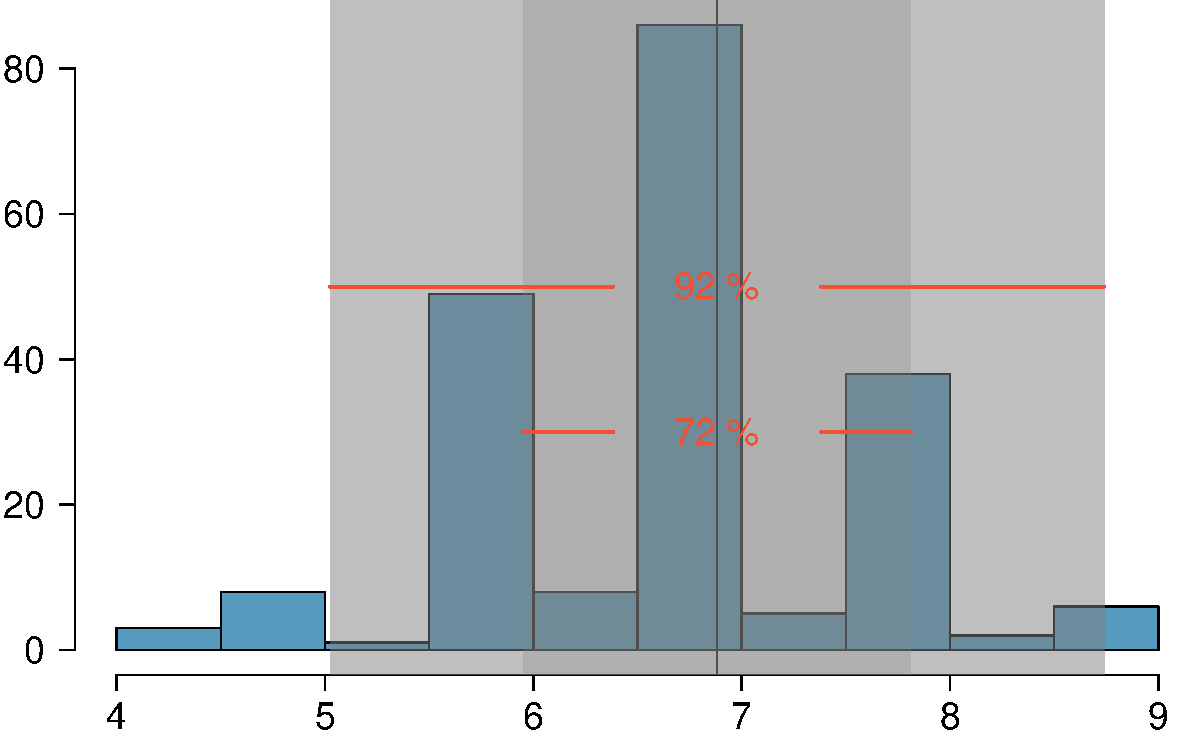
\includegraphics[width=0.75\textwidth]{\chp4@path/4-1_normal_distribution/figures/sleep/sleep-hist-sd2} 
\end{center}
\vspace{-0.25cm}
\begin{itemize}
\item Mean = 6.88 hours, SD = 0.92 hrs
\item 72\% of the data are within 1 SD of the mean: $6.88 \pm 0.93$
\item 92\% of the data are within 1 SD of the mean: $6.88 \pm 2 \times 0.93$
\item[] \textcolor{white}{99\% of the data are within 3 SD of the mean: $6.88 \pm 3 \times 0.93$}
\end{itemize}
}

\only<4>{
\begin{center}
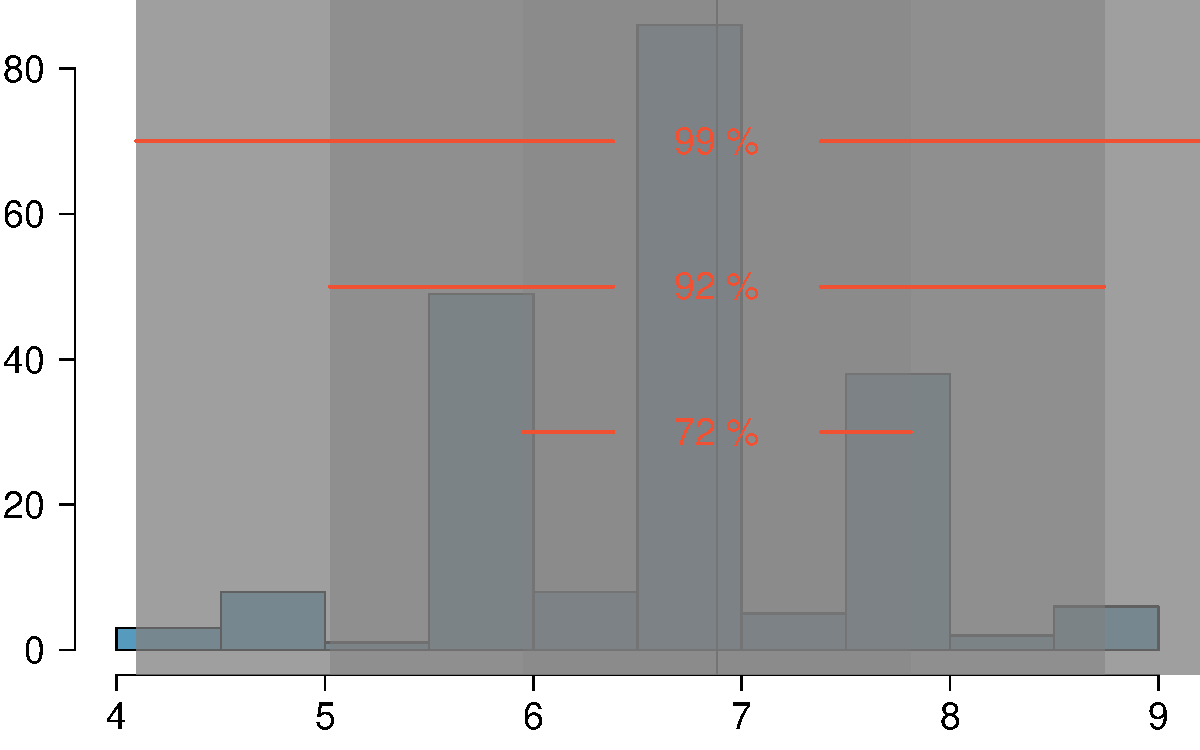
\includegraphics[width=0.75\textwidth]{\chp4@path/4-1_normal_distribution/figures/sleep/sleep-hist-sd3} 
\end{center}
\vspace{-0.25cm}
\begin{itemize}
\item Mean = 6.88 hours, SD = 0.92 hrs
\item 72\% of the data are within 1 SD of the mean: $6.88 \pm 0.93$
\item 92\% of the data are within 2 SD of the mean: $6.88 \pm 2 \times 0.93$
\item 99\% of the data are within 3 SD of the mean: $6.88 \pm 3 \times 0.93$
\end{itemize}
}

\end{frame}

%%%%%%%%%%%%%%%%%%%%%%%%%%%%%%%%%%%%

% \begin{frame}
% \frametitle{Practice}

% \pq{Which of the following is \underline{false}?}

% \begin{enumerate}[(a)]
% \item Majority of Z scores in a right skewed distribution are negative.
% \solnMult{In skewed distributions the Z score of the mean might be different than 0.}
% \item For a normal distribution, IQR is less than $2 \times SD$.
% \item Z scores are helpful for determining how unusual a data point is compared to the rest of the data in the distribution.
% \end{enumerate}

% \end{frame}

%%%%%%%%%%%%%%%%%%%%%%%%%%%%%%%%%%%%

\section{R Demonstration: Variability with 68-95-99.7 rule}

%%%%%%%%%%%%%%%%%%%%%%%%%%%%%%%%%%%%

\section{Edfinity quiz: Variability, concept review}
% Thinking like the last Practice slide, commented out above  

%%%%%%%%%%%%%%%%%%%%%%%%%%%%%%%%%%%%
% End document
%%%%%%%%%%%%%%%%%%%%%%%%%%%%%%%%%%%%

\end{document}